\chapter{Einleitung}
\label{Kapitel Einleitung}


Dieses Handbuch erl�utert detailliert die Funktionen des Programms TEMPUS\raisebox{1ex}{\tiny \copyright} Version 2.0.

Das Programm wurde von Christian Paminger basierend auf XML entwickelt und programmiert.

TEMPUS\raisebox{1ex}{\tiny \copyright} ist ein Werkzeug zur Erstellung, Wartung und Modifikation von Stundenpl�nen an Hochschulen, insbesondere an Fachhochschulen und erlaubt es mehreren Usern gleichzeitig, an der selben Datenbank und dem selben Stundenplan zu arbeiten.
Die Bearbeitung erfolgt wochenweise basierend auf Kalenderwochen.
Die Steuerung geschieht haupts�chlich per Drag\&Drop.

Es ist darauf zu achten, dass derzeit noch keine vollst�ndige ''R�ckg�ngig-Funktion'' in das Programm integriert wurde. Alle �nderungen werden sofort in die Datenbank �bernommen und k�nnen nur schwer rekonstruiert werden.

TEMPUS\raisebox{1ex}{\tiny \copyright}  arbeitet mit zwei Datenbanktabellen, die sich in regelm��igen Abst�nden synchronisieren.
Gearbeitet wird in erster Linie auf der Tabelle ''Stundenplandev'' (Entwicklungsoberfl�che), die jede Nacht in die Tabelle ''Stundenplan'' kopiert wird.
Die Tabelle ''Stundenplan'' ist die Onlinetabelle, die von Studenten und Lektoren abgerufen wird.
Bis zu einem gewissen Grad erlaubt diese Absicherung ein Wiederherstellen von gel�schten Daten.
Dennoch sollte die Stundenplanung sorgf�ltig und �berlegt  durchgef�hrt werden, da eine Rekonstruktion der Daten schwierig ist. Gerade beim L�schen von Daten ist dies ratsam.
Dieser Aufbau ist dar�ber hinaus die Basis f�r die automatische Infomail, die beim Synchronisieren alle �nderungen an die betroffenen Studenten und Lektoren kommuniziert.


\begin {figure}
	\centering
	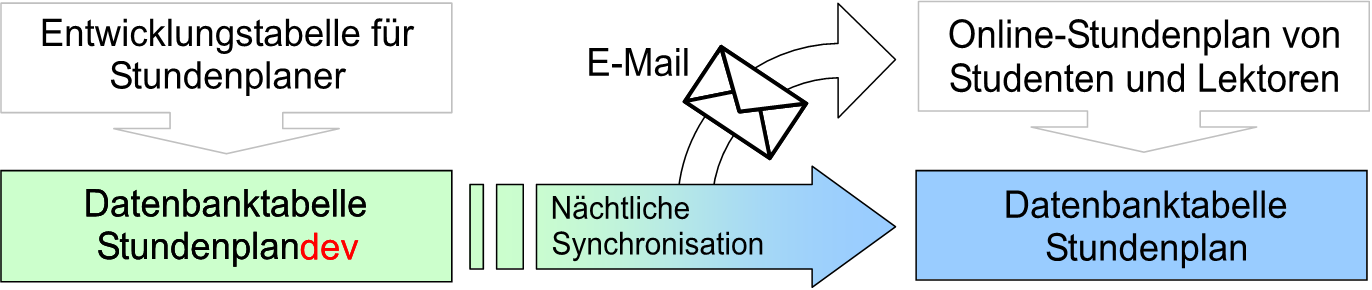
\includegraphics[width=1.0\textwidth]{SynchroSchema}
	%\caption{LE-Eigenschaften}
	\label{Schema}
\end {figure}

\achtung{�nderungen in der Onlinetabelle werden nicht in die Entwicklungsoberfl�che �bernommen. Deshalb m�ssen Sie dringende �nderungen immer in beiden Tabellen durchf�hren.
Es werden jede Nacht nur die Daten der Tabelle ''Stundenplandev'' �bernommen!}

\info{Auf Grund von unterschiedlichen Berechtigungen sind eventuell nicht alle in diesem Handbuch beschriebenen Features verf�gbar}
